\section{Selection Cuts for TauTau Channel}
\label{sect:tauTauCuts}
\subsection{pre-selection}
In the context of MSSM, supersymmetric objects are produced in pairs to conserve R-parity quantum number. Therefore in the production of charginos from proton-proton collisions, one may consider the following interaction $$pp\rightarrow\tilde{\chi_{1}^{+}}\tilde{\chi_{1}^{-}}\rightarrow\tilde{\tau}^{+}\nu \tilde{\tau}^{-}\nu\rightarrow\tau^{+}\tilde{\chi_{1}^{0}}\nu\tau^{-}\tilde{\chi_{1}^{0}}\nu\rightarrow\tau^{+}\tau^{-} + 2\tilde{\chi_{1}^{0}} + 2\nu.$$ In the detector, what can be observed are only 2 tau leptons plus missing transverse energy from the presence of neturinos and neutralinos in the final state.\\
The tau leptons can decay leptonically, in 35\% of the time, or can decay via hadrons, which is occuring with 65\% of probability. Since there are two leptons in the final state, then the probability of having $\tilde{\chi_{1}^{+}}\tilde{\chi_{1}^{-}} \rightarrow \tau_h+e/\mu+E_{T}^{miss}$ is about 46\%, while the probability of occuring $\tilde{\chi_{1}^{+}}\tilde{\chi_{1}^{-}} \rightarrow \tau_h+\tau_h+E_{T}^{miss}$ is about 42\%. Hereafter, final states containing a lepton are referred to as $e/\mu\text{-}\tau_h$ channel and those events where the two taus decays via hadrons are referred to as $di\text{-}\tau_h$. This section describes the cuts to enhance $di\text{-}\tau_h$ events. The list of cuts to select the $e/\mu\text{-}\tau_h$ events can be found in Section~\ref{sect:eleTauCuts} and ~\ref{sect:muTauCuts}.\\    
In the final state with 2 hadronic taus, events are required to pass the following list of cuts
\begin{itemize}
\item at least two reconstructed opposit-sign tau objects, with $p_T>45GeV$ and $|\eta|<2.1$, are required;\\ Since the online trigger cuts require two taus with $p_T>35GeV$, then it can be justified to have an offline cut on $p_T>45GeV$. 
\item both taus are required to pass medium isolation criteria;\\ In the online selection, it is also required two medium isolated taus.
\item extra muons and leptons are vetoed;\\ In order to reject background from di-boson events, events with extra leptons are failed for further analysis.
\item the invariant mass of the two taus, $M_{\tau\tau}$, should be above 12 GeV;\\ This cut removes backgrounds from multi-jet events. 
\item events under the Z mass peak are rejected, namely $|M_{\tau\tau}-M_Z^{rec}|>15GeV$;\\ This requirement acts against DY background events. 
\item A cut on $min\Delta\phi$ is applied to be above 1;\\ This cut is introduced against multi-jet events.   
\item $M_{T2}>40GeV$. 
\end{itemize}
\subsection{selection}
After applying pre-selection cuts, two extra set of cuts are introduced, where each of them is sensitive to some regions of $\chi_{1}^{\pm}\chi_{1}^{0}$ mass plane: one aimed the regions with large mass difference between charginos and neutralinos, the other one is dedicated for low mass regions. It should be noted that the two search bins are chosen to be exclusive in order to be able to combine the statistics at the end.
\subsubsection{search bin\#1: sensitive to high $\Delta M$}
A first set of cuts includes a cut on $M_{T2}$.
\begin{itemize}
\item $M_{T2}>90GeV$.
\end{itemize}
\subsubsection{search bin\#2: sensitive to low $\Delta M$}
A second set of cuts includes some cuts on different variables listed below.
\begin{itemize}
\item $M_{T2}<90GeV$;
\item $\Sigma M_{\tau}>250GeV$;
\item b-jets tagged with $CSVM$ algorithm are vetoed.
\end{itemize}
\subsection{cut flow table}
Two cut flow tables according to each of search bins are presented, which can be found in Tables~\ref{tbl:cutflowtable1} and~\ref{tbl:cutflowtable2}. The SUSY signal points used in the tables and figures correspond to $(M_{\chi_{1}^{\pm}}=240GeV,M_{\chi_{1}^{0}}=40GeV)$.   
%\begin{sidewaystable}
\begin{table}
\begin{center}
\scalebox{1.3}{
\begin{tabular}{lcccccccc}
\hline\hline
  &SUSY&QCD&VV&Wtolnu&DY&Top&Total Bkg&\\
\hline\hline
pre-selection &10.90&135.29&1.11&31.93&13.17&5.26&186.76$\pm$135.47&\\
$M_{T2}>90$&4.10&0.00&0.02&0.00&0.56&0.00&0.58$\pm$0.07&\\
\hline\hline
\end{tabular}}
\caption{Cut-flow-table for di-$\tau_h$ channel: search bin\#1.}
\label{tbl:cutflowtable1}
\scalebox{1.3}{
\begin{tabular}{lcccccccc}
\hline\hline
  &SUSY&QCD&VV&Wtolnu&DY&Top&Total Bkg&\\
\hline\hline
pre-selection &10.90&135.29&1.11&31.93&13.17&5.26&186.76$\pm$135.47&\\
$M_{T2} < $ 90 &6.80&135.29&1.09&31.93&12.60&5.26&186.17$\pm$135.47&\\
$\Sigma M_T^{\tau_i} > $ 250 &3.85&0.00&0.23&1.02&0.83&2.63&4.71$\pm$1.49&\\
b-jet veto &3.13&0.00&0.15&0.43&0.81&0.53&1.91$\pm$0.87&\\
\hline\hline
\end{tabular}}
\caption{Cut-flow-table for di-$\tau_h$ channel: search bin\#2.}
\label{tbl:cutflowtable2}
\end{center}
\end{table}
%\end{sidewaystable}
\subsection{data-MC comparison}
The distributions of $M_{T2}$ and $\Sigma M_T$ after applying pre-selection cuts are shown in Figure~\ref{fig:comparison}. There is only one QCD event with slightly large weight contributing to the plots. Hence the disagreement between data and MC in a couple of bins of $\Sigma M_T$ distribution can be justifed. In order to be blind to data, in both distributions data events are not shown at some points. Overally, it can be concluded that data and MC are in reasonable agreement. 
\begin{figure}[htbp]
\centering
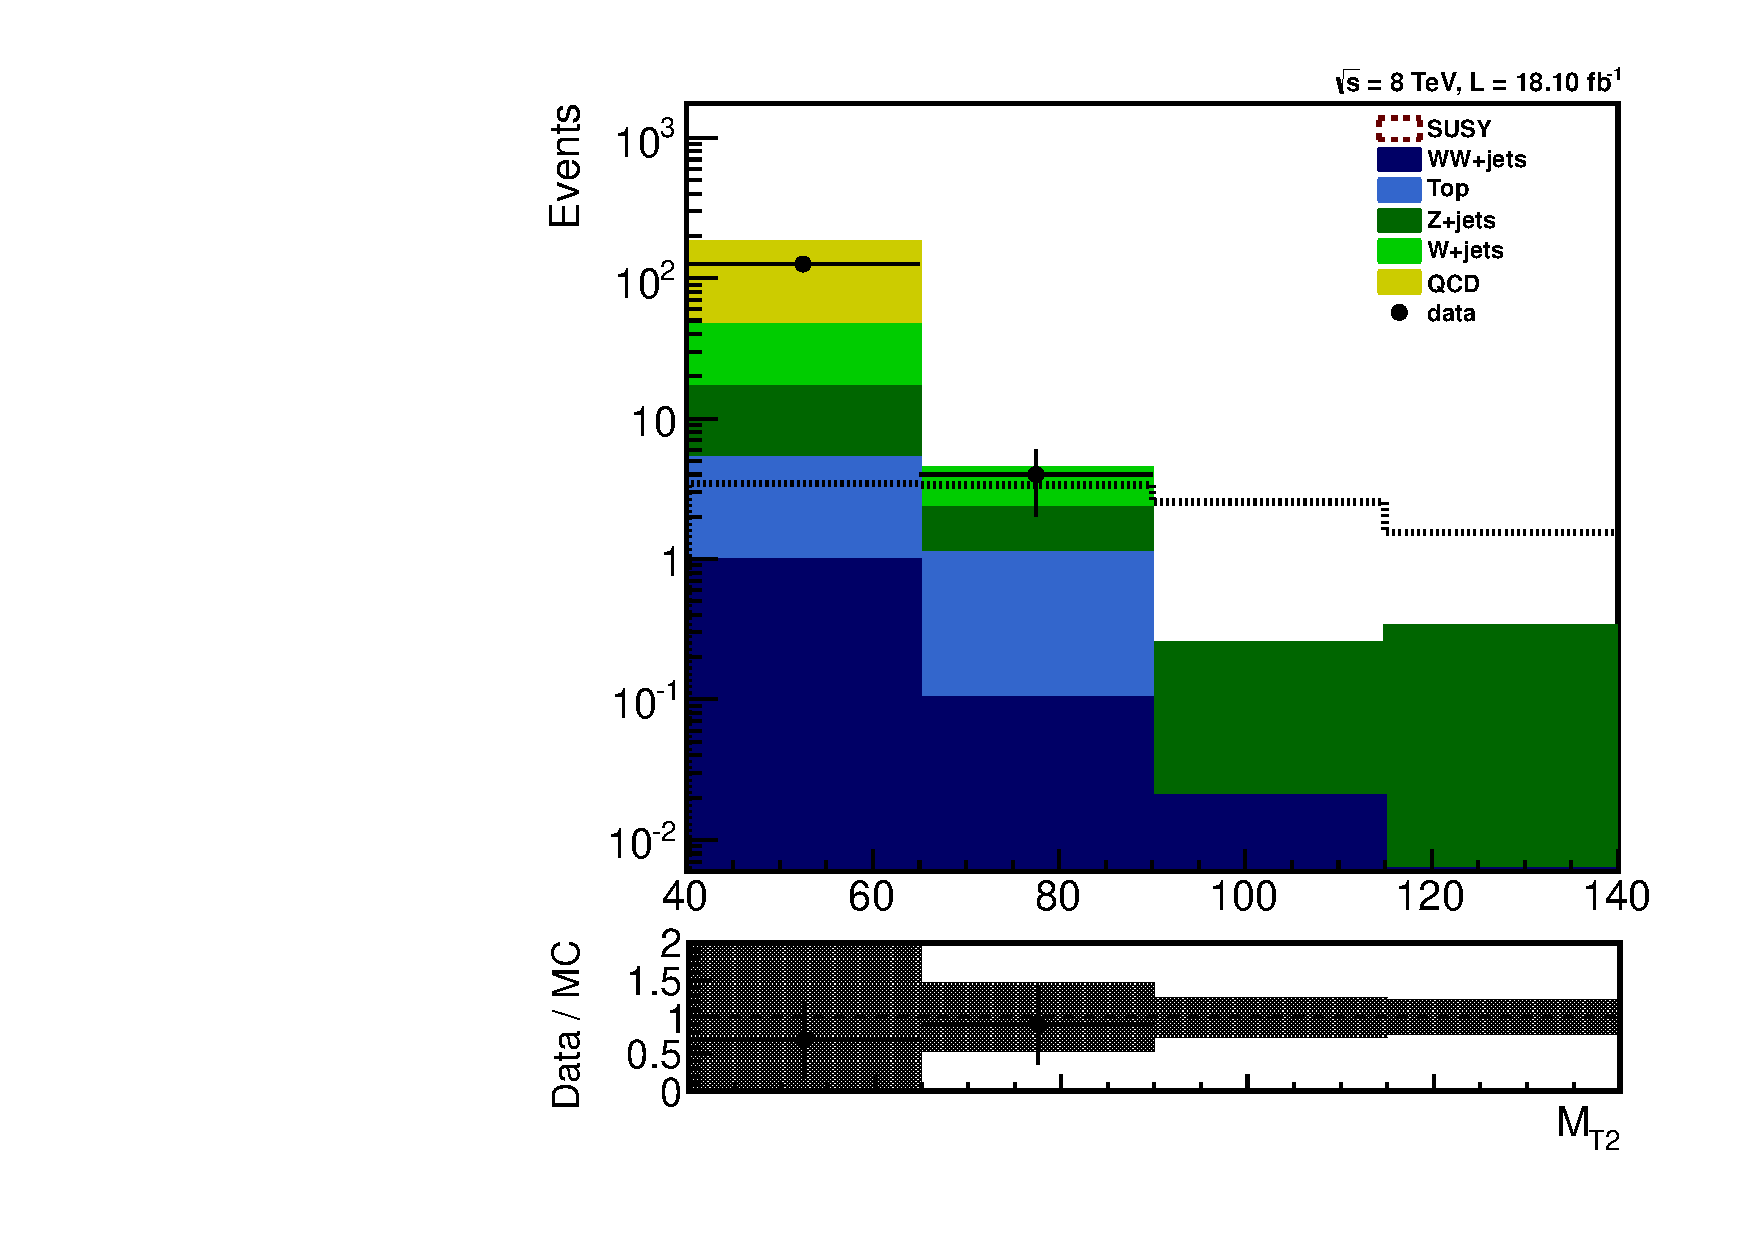
\includegraphics[angle=0,scale=0.35]{TauTauFigs/MT2_4bins.pdf}
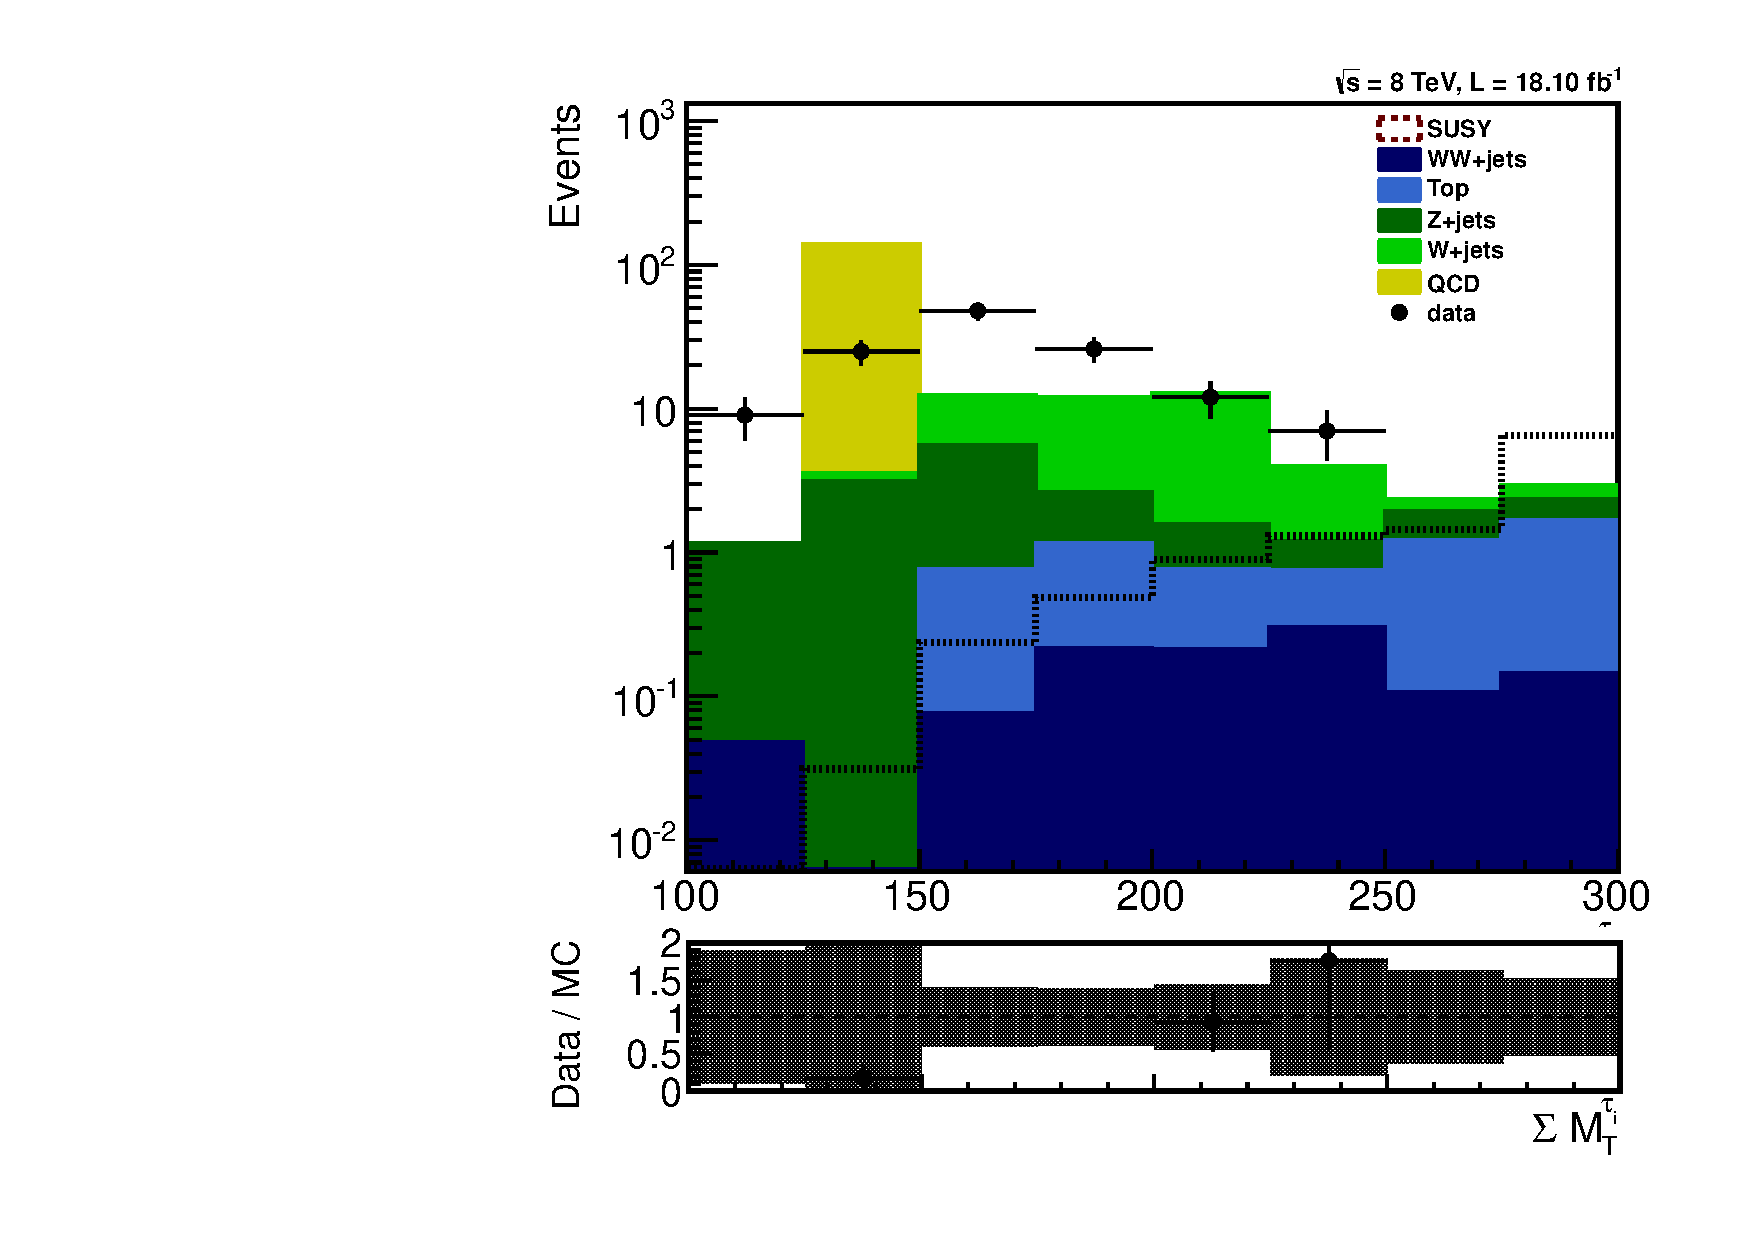
\includegraphics[angle=0,scale=0.35]{TauTauFigs/SumMT_8bins.pdf} \\
\caption{Left: MT2. Right: SumMT.}
\label{fig:comparison}
\end{figure}
\subsection{DY background estimation}
\subsection{exclusion limit}
\begin{figure}[htbp]
\centering
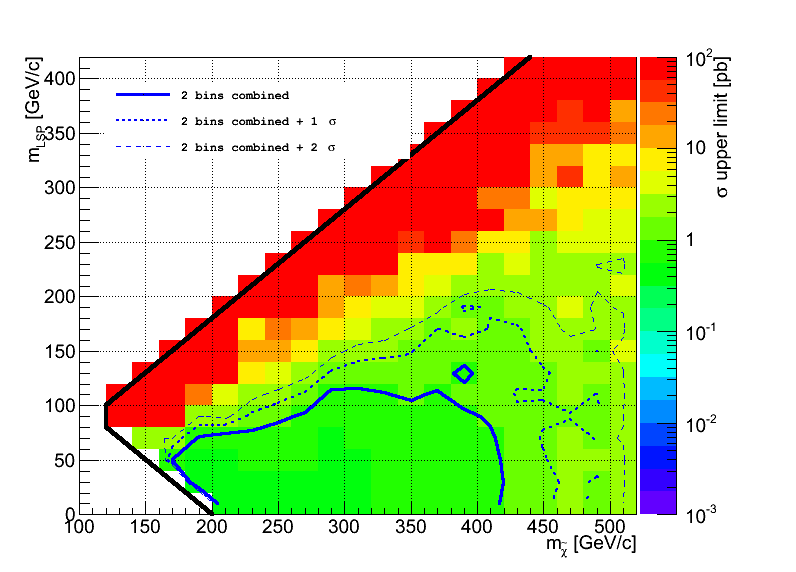
\includegraphics[angle=0,scale=0.35]{TauTauFigs/diTau_exclusion.png}
\caption{Exclusion limit plot.}
\label{fig:comparison}
\end{figure}
